\documentclass{standalone}
\usepackage{tikz}
\usetikzlibrary{patterns, positioning}


\begin{document}
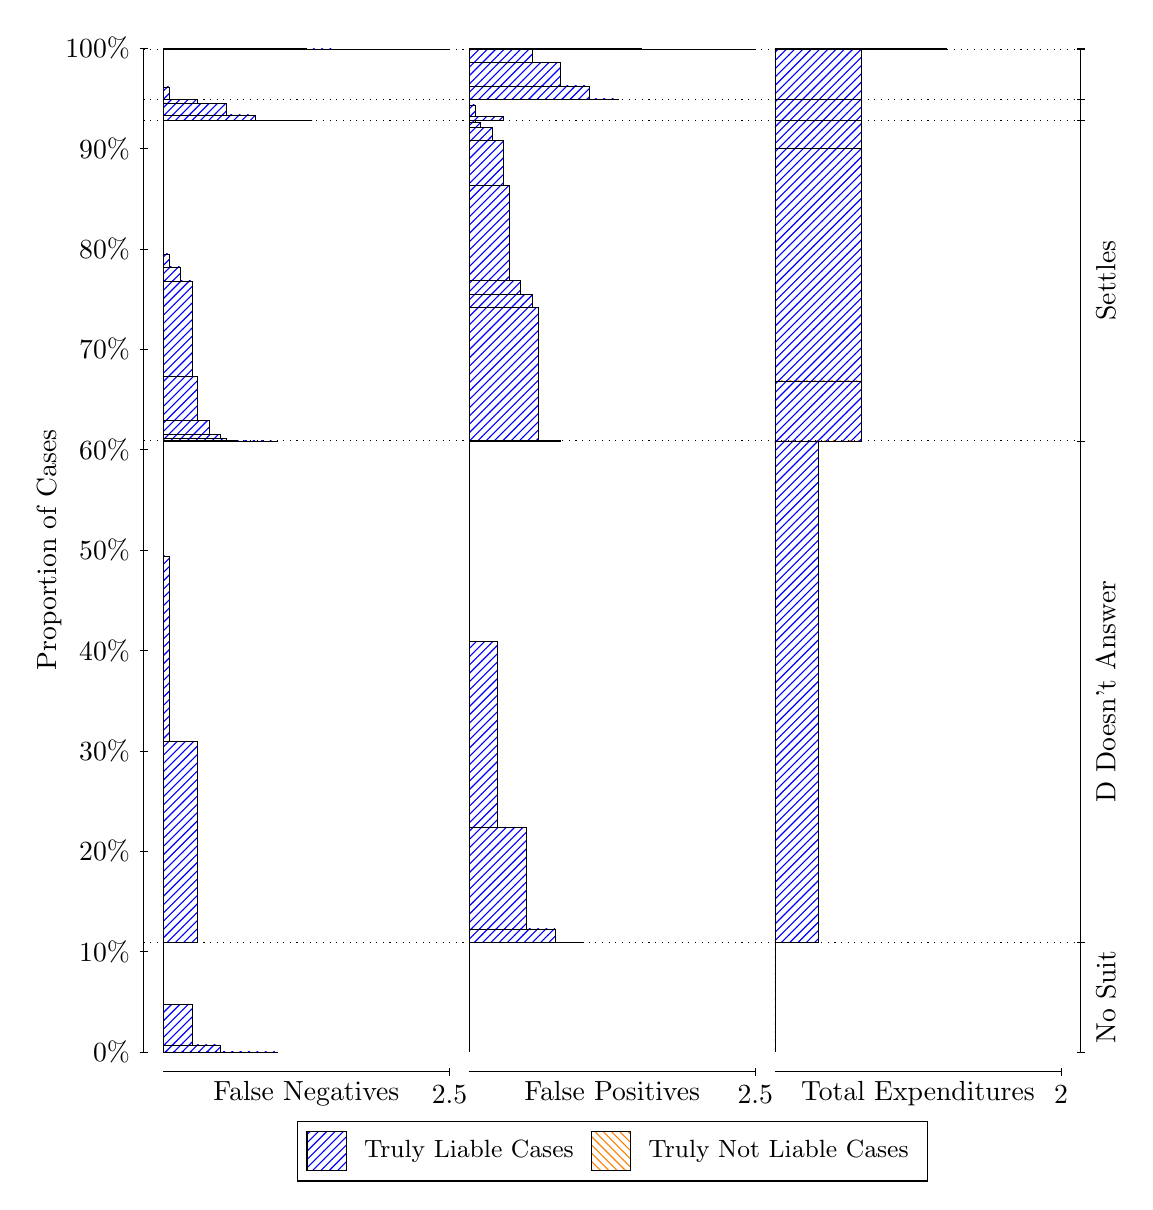
\begin{tikzpicture}
\draw[black, very thin] (1.5,1.75) -- (1.5,14.5);
\node[rotate=90, text=black, anchor=center] at (0.3, 8.125) {Proportion of Cases};
\draw[black, very thin] (1.45,1.75) -- (1.55,1.75);
\node[text=black, anchor=east] at (1.45, 1.75) {0\%};
\draw[black, very thin] (1.45,3.025) -- (1.55,3.025);
\node[text=black, anchor=east] at (1.45, 3.025) {10\%};
\draw[black, very thin] (1.45,4.3) -- (1.55,4.3);
\node[text=black, anchor=east] at (1.45, 4.3) {20\%};
\draw[black, very thin] (1.45,5.575) -- (1.55,5.575);
\node[text=black, anchor=east] at (1.45, 5.575) {30\%};
\draw[black, very thin] (1.45,6.85) -- (1.55,6.85);
\node[text=black, anchor=east] at (1.45, 6.85) {40\%};
\draw[black, very thin] (1.45,8.125) -- (1.55,8.125);
\node[text=black, anchor=east] at (1.45, 8.125) {50\%};
\draw[black, very thin] (1.45,9.4) -- (1.55,9.4);
\node[text=black, anchor=east] at (1.45, 9.4) {60\%};
\draw[black, very thin] (1.45,10.675) -- (1.55,10.675);
\node[text=black, anchor=east] at (1.45, 10.675) {70\%};
\draw[black, very thin] (1.45,11.95) -- (1.55,11.95);
\node[text=black, anchor=east] at (1.45, 11.95) {80\%};
\draw[black, very thin] (1.45,13.225) -- (1.55,13.225);
\node[text=black, anchor=east] at (1.45, 13.225) {90\%};
\draw[black, very thin] (1.45,14.5) -- (1.55,14.5);
\node[text=black, anchor=east] at (1.45, 14.5) {100\%};

\draw[black, very thin] (13.4,1.75) -- (13.4,14.5);
\draw[black, very thin] (13.35,1.75) -- (13.45,1.75);
\node[anchor=west] at (13.35, 1.75) {};
\draw[black, very thin] (13.35,3.1426) -- (13.45,3.1426);
\node[anchor=west] at (13.35, 3.1426) {};
\draw[black, very thin] (13.35,9.5102) -- (13.45,9.5102);
\node[anchor=west] at (13.35, 9.5102) {};
\draw[black, very thin] (13.35,13.583) -- (13.45,13.583);
\node[anchor=west] at (13.35, 13.583) {};
\draw[black, very thin] (13.35,13.846) -- (13.45,13.846);
\node[anchor=west] at (13.35, 13.846) {};
\draw[black, very thin] (13.35,14.483) -- (13.45,14.483);
\node[anchor=west] at (13.35, 14.483) {};
\draw[black, very thin] (13.35,14.5) -- (13.45,14.5);
\node[anchor=west] at (13.35, 14.5) {};

\draw[black, very thin, pattern color=blue, pattern=north east lines] (1.75,1.75) rectangle (3.2033,1.75);
\draw[black, very thin, pattern color=blue, pattern=north east lines] (1.75,1.75) rectangle (2.84,1.7507);
\draw[black, very thin, pattern color=blue, pattern=north east lines] (1.75,1.7507) rectangle (2.4767,1.8387);
\draw[black, very thin, pattern color=blue, pattern=north east lines] (1.75,1.8387) rectangle (2.1133,2.3497);
\draw[black, very thin, pattern color=orange, pattern=north west lines] (1.75,2.3497) rectangle (1.75,2.3497);
\draw[black, very thin, pattern color=blue, pattern=north east lines] (1.75,2.3497) rectangle (1.75,3.1426);
\draw[black, very thin, pattern color=blue, pattern=north east lines] (1.75,3.1426) rectangle (2.186,5.6906);
\draw[black, very thin, pattern color=blue, pattern=north east lines] (1.75,5.6906) rectangle (1.8227,8.0505);
\draw[black, very thin, pattern color=orange, pattern=north west lines] (1.75,8.0505) rectangle (1.75,8.0505);
\draw[black, very thin, pattern color=blue, pattern=north east lines] (1.75,8.0505) rectangle (1.75,9.5102);
\draw[black, very thin, pattern color=blue, pattern=north east lines] (1.75,9.5102) rectangle (3.2033,9.5102);
\draw[black, very thin, pattern color=blue, pattern=north east lines] (1.75,9.5102) rectangle (3.058,9.5102);
\draw[black, very thin, pattern color=blue, pattern=north east lines] (1.75,9.5102) rectangle (2.9127,9.5102);
\draw[black, very thin, pattern color=blue, pattern=north east lines] (1.75,9.5102) rectangle (2.84,9.5102);
\draw[black, very thin, pattern color=blue, pattern=north east lines] (1.75,9.5102) rectangle (2.6947,9.5141);
\draw[black, very thin, pattern color=blue, pattern=north east lines] (1.75,9.5141) rectangle (2.5493,9.5399);
\draw[black, very thin, pattern color=blue, pattern=north east lines] (1.75,9.5399) rectangle (2.4767,9.5981);
\draw[black, very thin, pattern color=blue, pattern=north east lines] (1.75,9.5981) rectangle (2.3313,9.7681);
\draw[black, very thin, pattern color=blue, pattern=north east lines] (1.75,9.7681) rectangle (2.186,10.334);
\draw[black, very thin, pattern color=blue, pattern=north east lines] (1.75,10.334) rectangle (2.1133,11.542);
\draw[black, very thin, pattern color=blue, pattern=north east lines] (1.75,11.542) rectangle (1.968,11.72);
\draw[black, very thin, pattern color=blue, pattern=north east lines] (1.75,11.72) rectangle (1.8227,11.886);
\draw[black, very thin, pattern color=orange, pattern=north west lines] (1.75,11.886) rectangle (1.75,11.886);
\draw[black, very thin, pattern color=blue, pattern=north east lines] (1.75,11.886) rectangle (1.75,13.583);
\draw[black, very thin, pattern color=blue, pattern=north east lines] (1.75,13.583) rectangle (3.6393,13.583);
\draw[black, very thin, pattern color=blue, pattern=north east lines] (1.75,13.583) rectangle (3.276,13.583);
\draw[black, very thin, pattern color=blue, pattern=north east lines] (1.75,13.583) rectangle (2.9127,13.65);
\draw[black, very thin, pattern color=blue, pattern=north east lines] (1.75,13.65) rectangle (2.5493,13.797);
\draw[black, very thin, pattern color=blue, pattern=north east lines] (1.75,13.797) rectangle (2.186,13.846);
\draw[black, very thin, pattern color=orange, pattern=north west lines] (1.75,13.846) rectangle (1.75,13.846);
\draw[black, very thin, pattern color=blue, pattern=north east lines] (1.75,13.846) rectangle (2.186,13.848);
\draw[black, very thin, pattern color=blue, pattern=north east lines] (1.75,13.848) rectangle (1.8227,14.007);
\draw[black, very thin, pattern color=orange, pattern=north west lines] (1.75,14.007) rectangle (1.75,14.007);
\draw[black, very thin, pattern color=blue, pattern=north east lines] (1.75,14.007) rectangle (1.75,14.483);
\draw[black, very thin, pattern color=blue, pattern=north east lines] (1.75,14.483) rectangle (5.3833,14.483);
\draw[black, very thin, pattern color=blue, pattern=north east lines] (1.75,14.483) rectangle (5.02,14.483);
\draw[black, very thin, pattern color=blue, pattern=north east lines] (1.75,14.483) rectangle (4.6567,14.483);
\draw[black, very thin, pattern color=blue, pattern=north east lines] (1.75,14.483) rectangle (4.2933,14.487);
\draw[black, very thin, pattern color=blue, pattern=north east lines] (1.75,14.487) rectangle (3.93,14.49);
\draw[black, very thin, pattern color=blue, pattern=north east lines] (1.75,14.49) rectangle (3.5667,14.491);
\draw[black, very thin, pattern color=blue, pattern=north east lines] (1.75,14.491) rectangle (2.404,14.491);
\draw[black, very thin, pattern color=blue, pattern=north east lines] (1.75,14.491) rectangle (2.0407,14.491);
\draw[black, very thin, pattern color=orange, pattern=north west lines] (1.75,14.491) rectangle (1.75,14.491);
\draw[black, very thin, pattern color=blue, pattern=north east lines] (1.75,14.491) rectangle (1.75,14.5);
\draw[black, very thin, pattern color=orange, pattern=north west lines] (5.6333,1.75) rectangle (5.6333,1.75);
\draw[black, very thin, pattern color=blue, pattern=north east lines] (5.6333,1.75) rectangle (5.6333,3.1426);
\draw[black, very thin, pattern color=orange, pattern=north west lines] (5.6333,3.1426) rectangle (7.0867,3.1426);
\draw[black, very thin, pattern color=blue, pattern=north east lines] (5.6333,3.1426) rectangle (7.0867,3.144);
\draw[black, very thin, pattern color=blue, pattern=north east lines] (5.6333,3.144) rectangle (6.7233,3.3133);
\draw[black, very thin, pattern color=blue, pattern=north east lines] (5.6333,3.3133) rectangle (6.36,4.6022);
\draw[black, very thin, pattern color=blue, pattern=north east lines] (5.6333,4.6022) rectangle (5.9967,6.9622);
\draw[black, very thin, pattern color=blue, pattern=north east lines] (5.6333,6.9622) rectangle (5.6333,9.5102);
\draw[black, very thin, pattern color=orange, pattern=north west lines] (5.6333,9.5102) rectangle (6.796,9.5102);
\draw[black, very thin, pattern color=blue, pattern=north east lines] (5.6333,9.5102) rectangle (6.796,9.5148);
\draw[black, very thin, pattern color=orange, pattern=north west lines] (5.6333,9.5148) rectangle (6.6507,9.5148);
\draw[black, very thin, pattern color=blue, pattern=north east lines] (5.6333,9.5148) rectangle (6.6507,9.5204);
\draw[black, very thin, pattern color=orange, pattern=north west lines] (5.6333,9.5204) rectangle (6.5053,9.5204);
\draw[black, very thin, pattern color=blue, pattern=north east lines] (5.6333,9.5204) rectangle (6.5053,11.207);
\draw[black, very thin, pattern color=blue, pattern=north east lines] (5.6333,11.207) rectangle (6.4327,11.373);
\draw[black, very thin, pattern color=blue, pattern=north east lines] (5.6333,11.373) rectangle (6.2873,11.552);
\draw[black, very thin, pattern color=blue, pattern=north east lines] (5.6333,11.552) rectangle (6.142,12.759);
\draw[black, very thin, pattern color=blue, pattern=north east lines] (5.6333,12.759) rectangle (6.0693,13.325);
\draw[black, very thin, pattern color=blue, pattern=north east lines] (5.6333,13.325) rectangle (5.924,13.495);
\draw[black, very thin, pattern color=blue, pattern=north east lines] (5.6333,13.495) rectangle (5.7787,13.553);
\draw[black, very thin, pattern color=blue, pattern=north east lines] (5.6333,13.553) rectangle (5.706,13.579);
\draw[black, very thin, pattern color=blue, pattern=north east lines] (5.6333,13.579) rectangle (5.6333,13.583);
\draw[black, very thin, pattern color=orange, pattern=north west lines] (5.6333,13.583) rectangle (6.0693,13.583);
\draw[black, very thin, pattern color=blue, pattern=north east lines] (5.6333,13.583) rectangle (6.0693,13.631);
\draw[black, very thin, pattern color=blue, pattern=north east lines] (5.6333,13.631) rectangle (5.706,13.779);
\draw[black, very thin, pattern color=blue, pattern=north east lines] (5.6333,13.779) rectangle (5.6333,13.846);
\draw[black, very thin, pattern color=orange, pattern=north west lines] (5.6333,13.846) rectangle (7.5227,13.846);
\draw[black, very thin, pattern color=blue, pattern=north east lines] (5.6333,13.846) rectangle (7.5227,13.855);
\draw[black, very thin, pattern color=blue, pattern=north east lines] (5.6333,13.855) rectangle (7.1593,14.02);
\draw[black, very thin, pattern color=blue, pattern=north east lines] (5.6333,14.02) rectangle (6.796,14.322);
\draw[black, very thin, pattern color=blue, pattern=north east lines] (5.6333,14.322) rectangle (6.4327,14.481);
\draw[black, very thin, pattern color=blue, pattern=north east lines] (5.6333,14.481) rectangle (6.0693,14.483);
\draw[black, very thin, pattern color=orange, pattern=north west lines] (5.6333,14.483) rectangle (9.2667,14.483);
\draw[black, very thin, pattern color=blue, pattern=north east lines] (5.6333,14.483) rectangle (9.2667,14.483);
\draw[black, very thin, pattern color=orange, pattern=north west lines] (5.6333,14.483) rectangle (8.9033,14.483);
\draw[black, very thin, pattern color=blue, pattern=north east lines] (5.6333,14.483) rectangle (8.9033,14.483);
\draw[black, very thin, pattern color=orange, pattern=north west lines] (5.6333,14.483) rectangle (8.54,14.483);
\draw[black, very thin, pattern color=blue, pattern=north east lines] (5.6333,14.483) rectangle (8.54,14.484);
\draw[black, very thin, pattern color=orange, pattern=north west lines] (5.6333,14.484) rectangle (8.1767,14.484);
\draw[black, very thin, pattern color=blue, pattern=north east lines] (5.6333,14.484) rectangle (8.1767,14.487);
\draw[black, very thin, pattern color=blue, pattern=north east lines] (5.6333,14.487) rectangle (7.8133,14.492);
\draw[black, very thin, pattern color=blue, pattern=north east lines] (5.6333,14.492) rectangle (7.45,14.493);
\draw[black, very thin, pattern color=blue, pattern=north east lines] (5.6333,14.493) rectangle (7.0867,14.493);
\draw[black, very thin, pattern color=blue, pattern=north east lines] (5.6333,14.493) rectangle (6.7233,14.493);
\draw[black, very thin, pattern color=orange, pattern=north west lines] (5.6333,14.493) rectangle (5.6333,14.493);
\draw[black, very thin, pattern color=blue, pattern=north east lines] (5.6333,14.493) rectangle (5.6333,14.5);
\draw[black, very thin, pattern color=orange, pattern=north west lines] (9.5167,1.75) rectangle (9.5167,1.75);
\draw[black, very thin, pattern color=blue, pattern=north east lines] (9.5167,1.75) rectangle (9.5167,3.1426);
\draw[black, very thin, pattern color=orange, pattern=north west lines] (9.5167,3.1426) rectangle (10.062,3.1426);
\draw[black, very thin, pattern color=blue, pattern=north east lines] (9.5167,3.1426) rectangle (10.062,9.5102);
\draw[black, very thin, pattern color=orange, pattern=north west lines] (9.5167,9.5102) rectangle (10.607,9.5102);
\draw[black, very thin, pattern color=blue, pattern=north east lines] (9.5167,9.5102) rectangle (10.607,10.272);
\draw[black, very thin, pattern color=orange, pattern=north west lines] (9.5167,10.272) rectangle (10.607,10.272);
\draw[black, very thin, pattern color=blue, pattern=north east lines] (9.5167,10.272) rectangle (10.607,13.225);
\draw[black, very thin, pattern color=orange, pattern=north west lines] (9.5167,13.225) rectangle (10.607,13.225);
\draw[black, very thin, pattern color=blue, pattern=north east lines] (9.5167,13.225) rectangle (10.607,13.583);
\draw[black, very thin, pattern color=orange, pattern=north west lines] (9.5167,13.583) rectangle (10.607,13.583);
\draw[black, very thin, pattern color=blue, pattern=north east lines] (9.5167,13.583) rectangle (10.607,13.846);
\draw[black, very thin, pattern color=orange, pattern=north west lines] (9.5167,13.846) rectangle (10.607,13.846);
\draw[black, very thin, pattern color=blue, pattern=north east lines] (9.5167,13.846) rectangle (10.607,14.483);
\draw[black, very thin, pattern color=orange, pattern=north west lines] (9.5167,14.483) rectangle (11.697,14.483);
\draw[black, very thin, pattern color=blue, pattern=north east lines] (9.5167,14.483) rectangle (11.697,14.5);
\draw[black, dotted] (1.5,3.1426) -- (13.4,3.1426);
\draw[black, dotted] (1.5,9.5102) -- (13.4,9.5102);
\draw[black, dotted] (1.5,13.583) -- (13.4,13.583);
\draw[black, dotted] (1.5,13.846) -- (13.4,13.846);
\draw[black, dotted] (1.5,14.483) -- (13.4,14.483);
\draw[black, very thin] (1.75,1.5) -- (5.3833,1.5);
\node[text=black, anchor=north] at (3.5667, 1.5) {False Negatives};
\draw[black, very thin] (5.3833,1.45) -- (5.3833,1.55);
\node[text=black, anchor=north] at (5.3833, 1.45) {2.5};

\draw[black, very thin] (5.6333,1.5) -- (9.2667,1.5);
\node[text=black, anchor=north] at (7.45, 1.5) {False Positives};
\draw[black, very thin] (9.2667,1.45) -- (9.2667,1.55);
\node[text=black, anchor=north] at (9.2667, 1.45) {2.5};

\draw[black, very thin] (9.5167,1.5) -- (13.15,1.5);
\node[text=black, anchor=north] at (11.333, 1.5) {Total Expenditures};
\draw[black, very thin] (13.15,1.45) -- (13.15,1.55);
\node[text=black, anchor=north] at (13.15, 1.45) {2};

\node[text=black, centered, rotate=90] at (13.72, 2.4463) {No Suit};
\node[text=black, centered, rotate=90] at (13.72, 6.3264) {D Doesn't Answer};
\node[text=black, centered, rotate=90] at (13.72, 11.547) {Settles};




\draw (7.449999999999999,1.5) node[draw=none] (baseCoordinate) {};
\begin{scope}[align=center]
        \matrix[scale=0.5, draw=black, below=0.5cm of baseCoordinate, nodes={draw}, column sep=0.1cm]{
            \node[rectangle, draw, minimum width=0.5cm, minimum height=0.5cm, pattern color=blue, pattern=north east lines] {}; &
            \node[draw=none, font=\small, text=black] (B) {Truly Liable Cases}; &
            \node[rectangle, draw, minimum width=0.5cm, minimum height=0.5cm, pattern color=orange, pattern=north west lines] {}; &
            \node[draw=none, font=\small, text=black] (B) {Truly Not Liable Cases}; \\
            };
\end{scope}

\end{tikzpicture}
\end{document}